\documentclass[11pt]{ctexart}
\usepackage[top=2cm, bottom=2cm, left=2cm, right=2cm]{geometry}



\usepackage{algorithm,algpseudocode,float}
\makeatletter
\newenvironment{breakablealgorithm}
  {% \begin{breakablealgorithm}
   \begin{center}
     \refstepcounter{algorithm}% New algorithm
     \hrule height.8pt depth0pt \kern2pt% \@fs@pre for \@fs@ruled
     \renewcommand{\caption}[2][\relax]{% Make a new \caption
       {\raggedright\textbf{\ALG@name~\thealgorithm} ##2\par}%
       \ifx\relax##1\relax % #1 is \relax
         \addcontentsline{loa}{algorithm}{\protect\numberline{\thealgorithm}##2}%
       \else % #1 is not \relax
         \addcontentsline{loa}{algorithm}{\protect\numberline{\thealgorithm}##1}%
       \fi
       \kern2pt\hrule\kern2pt
     }
  }{% \end{breakablealgorithm}
     \kern2pt\hrule\relax% \@fs@post for \@fs@ruled
   \end{center}
  }
\makeatother

\usepackage{amsmath}
\usepackage{graphicx}
\usepackage{listings}
\usepackage{xcolor}
\usepackage{float}
\usepackage{amsmath}
\usepackage{amssymb}
\floatname{algorithm}{算法}
\renewcommand{\algorithmicrequire}{\textbf{输入:}}
\renewcommand{\algorithmicensure}{\textbf{输出:}}
\lstset{numbers=left, %设置行号位置
        numberstyle=\tiny, %设置行号大小
        keywordstyle=\color{blue}, %设置关键字颜色
        commentstyle=\color[cmyk]{1,0,1,0}, %设置注释颜色
        frame=single, %设置边框格式
        escapeinside=``, %逃逸字符(1左面的键),用于显示中文
        breaklines, %自动折行
        extendedchars=false, %解决代码跨页时,章节标题,页眉等汉字不显示的问题
        xleftmargin=2em,xrightmargin=2em, aboveskip=1em, %设置边距
        tabsize=4, %设置tab空格数
        showspaces=false %不显示空格
}
\title{\huge\bf
最长公共子序列 - 实验报告}
\author{毛圆鑫 - 201721012271}
\date{Nov 10, 2019}

\begin{document}  
\maketitle
\section*{说明}
本次代码不长,所以本文以完整的形式给出,但也请见所附的.cpp文件,

还有就是本文档是使用latex语言编写的,其源文件也可见于附件或Github,或https://github.com/punk-boy/algorithm/下的 longest\_common\_string.cpp

本次的动态规划问题,主要检查的逻辑的正确性,以及动态规划过程的理解,所以这次代码的测试用例为了简单化,均使用和老师一样的示例。


\section{伪代码}

\begin{breakablealgorithm}
\caption{最长公共子序列 - 动态规划解法 - 伪代码}
\begin{algorithmic}[1]
\Require 字符数组$X[]$,$Y[]$,动态规划数组$c[][]$,动态规划转移数组$b[][]$,$X$字符的长度$m$,$Y$字符的长度$n$
\Ensure 最长公共子序列的长度
\Function {LongestCommonString}{$X[],Y[],c[][],b[]][],m,n$}
\For{$i=0 \to m$}
\State $c[i][0] \gets 0$
\EndFor
\For{$j=0 \to n$}
$c[0][j] \gets 0$
\EndFor

\For{$i=0 \to m$}
\For{$j=0 \to n$}
	\If{$X[i] = Y[j]$}
		\State $c[i][j] = c[i-1][j-1]+1,b[i][j]='\nwarrow'$
	\ElsIf{$c[i-1][j] < c[i][j-1]$}
		\State $c[i][j]=c[i-1][j],b[i][j]='\uparrow'$
	\Else
		\State $c[i][j]=c[i][j-1],b[i][j]='\leftarrow'$
	\EndIf
\EndFor
\EndFor
\EndFunction
\end{algorithmic}
\end{breakablealgorithm}


\begin{algorithm}
\caption{回溯得到最长公共子序列 - 附加}
\begin{algorithmic}[1]
\Require 动态规划转移数组$b[][]$,字符数组$X[]$,$i$, $j$

\Function{PrintLCS}{$b[][],X[],i,j$}
\If{$i=0\quad or\quad j=0$}
	\Return{}
\EndIf
\If{$b[i][j]='\nwarrow'$}
	\State PrintLCS($b[][],x[],i-1,j-1$)
	\State print x[i]
\ElsIf{$b[i][j]='\uparrow'$}
	\State PrintLCS($b[][],x[],i-1,j$)
\Else
	\State PrintLCS($b[][],x[],i,j-1$)
\EndIf
\EndFunction

\end{algorithmic}

\end{algorithm}

\section{实现代码}
\begin{lstlisting}[language=C++]
#include <stdio.h>
#include <iostream>
#include <string.h>

#define N 100
int dp[N][N];
char b[N][N];

inline int max(int a, int b)
{
	return a>b?a:b;
}

inline int min(int a, int b)
{
	return a<b?a:b;
}

int longest_common_string(char * x, char * y, int m, int n)
{
	for(int i=0;i<=m;i++) dp[i][0] = 0;
	for(int j=0;j<=n;j++) dp[0][j] = 0;
	for(int i=1;i<=m;i++)
	{
		for(int j=1;j<=n;j++)
		{
			if(x[i-1] == y[j-1])
			{
				dp[i][j] = dp[i-1][j-1]+1;
				b[i][j] = 'O';
			}
			else if(dp[i-1][j] >= dp[i][j-1])
			{
				dp[i][j] = dp[i-1][j];
				b[i][j] = 'U';
			}
			else
			{
				dp[i][j] = dp[i][j-1];
				b[i][j] = 'L';
			}
		}
	}
	return dp[m][n];
}
void printLCS(char * x, int m, int n)
{
	if(m == 0 || n == 0)	
	{
		return ;
	}
	if(b[m][n] == 'O')
	{
		printLCS(x, m-1, n-1);
		printf("%c", x[m-1]);
	}
	else if(b[m][n] == 'U')
		printLCS(x, m-1, n);
	else if(b[m][n] == 'L')
		printLCS(x, m, n-1);
}
int main()
{
	int m = 7;
	int n = 6;
	char x[N] = "ABCBDAB";
	char y[N] = "BDCABA";
	printf("%s\n", x);
	printf("%s\n", y);
	int ret = longest_common_string(x, y, m, n);
	printf("---------------\n%d\n", ret);
	printLCS(x, m, n);
	printf("\n");
	return 0;
}
\end{lstlisting}

\section{实验结果}
\begin{figure}[H]
\centering
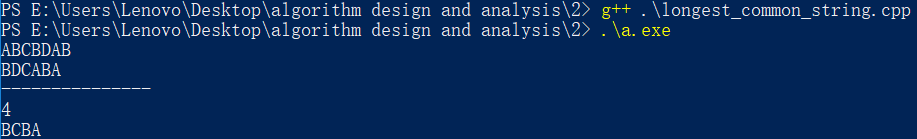
\includegraphics[scale=0.8]{longest_common_string.png}
\caption{最长公共子序列实验结果}
\label{Label_LCS}
\end{figure}

\end{document}



